\chapter{与学习相关的技巧}
本章将介绍神经网络的学习中的一些重要观点,主题涉及寻找最优权重
参数的最优化方法、权重参数的初始值、超参数的设定方法等。此外,为了
应对过拟合,本章还将介绍权值衰减、Dropout等正则化方法,并进行实现。
\section{参数的更新}
神经网络的学习的目的是找到使损失函数的值尽可能小的参数。这是寻
找最优参数的问题,解决这个问题的过程称为\textbf{最优化}(optimization)。遗憾的是,
神经网络的最优化问题非常难。这是因为参数空间非常复杂,无法轻易找到
最优解(无法使用那种通过解数学式一下子就求得最小值的方法)。而且,在
深度神经网络中,参数的数量非常庞大,导致最优化问题更加复杂。

使用参数的梯度,沿梯度方向更新参数,并重复这个步骤多次,从而逐渐靠
近最优参数,这个过程称为\textbf{随机梯度下降法}(stochastic gradient descent),
简称\textbf{SGD}。
\subsection{SGD}
用数学式可以将SGD写成如下式:
\begin{equation*}
    \bm{W}\leftarrow \bm{W}-\eta\frac{\partial L}{\partial \bm{W}}
\end{equation*}
SGD是朝着梯度方向只前进一定距离的简单方法。

\subsection{SGD的缺点}
虽然SGD简单,并且容易实现,但是在解决某些问题时可能没有效率。
\begin{equation*}
    z = \frac{1}{20}x^2+y^2
\end{equation*}
上式表示的函数是向 $x$ 轴方向延伸的“碗”状函数。

SGD的缺点是,如果函数的形状非均向(anisotropic),比如呈延伸状,搜索
的路径就会非常低效。因此,我们需要比单纯朝梯度方向前进的SGD更聪
明的方法。\important{SGD低效的根本原因是,梯度的方向并没有指向最小值的方向}。

\subsection{Momentum}
\begin{subequations}
    \begin{align}
        \bm{v} & \leftarrow  \alpha \bm{v}-\eta\frac{\partial L}{\partial \bm{W}} \label{eq11-a} \\
        \bm{W} & \leftarrow \bm{W}+\bm{v}\label{eq11-b}
    \end{align}
\end{subequations}
这里新出现了一个变量$\bm{v}$,对应物理上的速度。
\autoref{eq11-a}表示了物体在梯度方向上受力,在这个力的作用下,物体的速度增
加这一物理法则。如\autoref{Momentum-The ball rolls on an incline}所示,Momentum方法给人的感觉就像是小球在
地面上滚动。

式\autoref{eq11-a}中有$\alpha \bm{v}$这一项。在物体不受任何力时,该项承担使物体逐渐减
速的任务($\alpha$设定为0.9之类的值),对应物理上的地面摩擦或空气阻力。
\figures{Momentum-The ball rolls on an incline}
\subsection{AdaGrad}
在关于学习率的有效技巧中,有一种被称为\textbf{学习率衰减}(learning rate
decay)的方法,即随着学习的进行,使学习率逐渐减小。实际上,一开始“多”
学,然后逐渐“少”学的方法,在神经网络的学习中经常被使用。

逐渐减小学习率的想法,相当于将“全体”参数的学习率值一起降低。
而AdaGrad进一步发展了这个想法,针对“一个一个”的参数,赋予其“定
制”的值。AdaGrad会为参数的每个元素适当地调整学习率,与此同时进行学习。
\begin{subequations}
    \begin{align}
        \bm{h} & \leftarrow  \bm{h} + \frac{\partial L}{\partial \bm{W}} \odot \frac{\partial L}{\partial \bm{W}} \label{eq12-a} \\
        \bm{W} & \leftarrow \bm{W} -\eta \frac{1}{\sqrt{\bm{h}}}\frac{\partial L}{\partial \bm{W}} \label{eq12-b}
    \end{align}
\end{subequations}
式中,$\odot$表示对应矩阵元素的乘法,在更新参数时,通过乘以$\frac{1}{\sqrt{\bm{h}}}$
,就可以调整学习的尺度。这意味着,
参数的元素中变动较大(被大幅更新)的元素的学习率将变小。也就是说,
\important{可以按参数的元素进行学习率衰减,使变动大的参数的学习率逐渐减小}。
\begin{tcolorbox}
    \important{AdaGrad会记录过去所有梯度的平方和}。因此,学习越深入,更新
    的幅度就越小。实际上,如果无止境地学习,更新量就会变为 0,
    完全不再更新。为了改善这个问题,可以使用 RMSProp方法。
    RMSProp方法并不是将过去所有的梯度一视同仁地相加,而是逐渐
    地遗忘过去的梯度,在做加法运算时将新梯度的信息更多地反映出来。
    这种操作从专业上讲,称为“指数移动平均”,呈指数函数式地减小
    过去的梯度的尺度。
\end{tcolorbox}

\subsection{Adam}
\href{https://arxiv.org/abs/1412.6980v8}{Adam}是2015年提出的新方法。它的理论有些复杂,直观地讲,就是融
合了Momentum和AdaGrad的方法。通过组合前面两个方法的优点,有望
实现参数空间的高效搜索。此外,进行超参数的“偏置校正”也是Adam的特征。

\begin{tcolorbox}
    Adam会设置3个超参数。一个是学习率(论文中以$\alpha$出现),另外两
    个是一次momentum系数$\beta_1$和二次momentum系数$\beta_2$。根据论文,
    标准的设定值是$\beta_1$为0.9,$\beta_2$ 为0.999。设置了这些值后,大多数情
    况下都能顺利运行。
\end{tcolorbox}
\subsection{使用哪种更新方法呢}
\figures{Comparison of Optimization Methods}

如\autoref{Comparison of Optimization Methods}所示,根据使用的方法不同,参数更新的路径也不同。只看这
个图的话,AdaGrad似乎是最好的,不过也要注意,结果会根据要解决的问
题而变。并且,很显然,超参数(学习率等)的设定值不同,结果也会发生变化。

非常遗憾,(目前)并不存在能在所有问题中都表现良好
的方法。这4种方法各有各的特点,都有各自擅长解决的问题和不擅长解决
的问题。

\subsection{基于MNIST数据集的更新方法的比较}
\section{权重的初始值}
在神经网络的学习中,权重的初始值特别重要。实际上,设定什么样的
权重初始值,经常关系到神经网络的学习能否成功。

\subsection{可以将权重初始值设为0吗}
权值衰减(weights decay)就是一种以减小权重参数的值为目的进行学习
的方法。通过减小权重参数的值来抑制过拟合的发生。从结
论来说,将权重初始值设为0不是一个好主意。事实上,将权重初始值设为
0的话,将无法正确进行学习。

为了防止“权重均一化”
(严格地讲,是为了瓦解权重的对称结构),必须随机生成初始值。
\subsection{隐藏层的激活值的分布}
观察隐藏层的激活值\footnote{这里我们将激活函数的输出数据称为“激活值”,但是有的文献中会将在层之间流动的数据也称为“激
    活值”。}(激活函数的输出数据)的分布,可以获得很多启
发。
\figures{The distribution of the activation value of each layer when using a Gaussian distribution with a standard deviation of 1 as the initial weight value}
从\autoref{The distribution of the activation value of each layer when using a Gaussian distribution with a standard deviation of 1 as the initial weight value}可知,各层的激活值呈偏向0和1的分布。这里使用的sigmoid
函数是S型函数,随着输出不断地靠近0(或者靠近1),它的导数的值逐渐接
近0。因此,偏向0和1的数据分布会造成反向传播中梯度的值不断变小,最
后消失。这个问题称为梯度消失(gradient vanishing)。层次加深的深度学习
中,梯度消失的问题可能会更加严重。

\begin{tcolorbox}
    各层的激活值的分布都要求有适当的广度。为什么呢?因为通过
    在各层间传递多样性的数据,神经网络可以进行高效的学习。反
    过来,如果传递的是有所偏向的数据,就会出现梯度消失或者“表
    现力受限”的问题,导致学习可能无法顺利进行。
\end{tcolorbox}

Xavier的论文中,为了使各层的激活值呈现出具有相同广度的分布,推导了合适的权重尺度。推导出的结论是,如果前一层的节点数为$n$,则初始
值使用标准差为$\sqrt{\frac{1}{n}}$
的分布。

\figures{Xavier initial value}

使用Xavier初始值后的结果如\autoref{Distribution of activation values of each layer when using Xavier initial value as weight initial value}所示。从这个结果可知,越是后
面的层,图像变得越歪斜,但是呈现了比之前更有广度的分布。因为各层间
传递的数据有适当的广度,所以sigmoid函数的表现力不受限制,有望进行
高效的学习。

\begin{tcolorbox}
    \autoref{Distribution of activation values of each layer when using Xavier initial value as weight initial value}的分布中,后面的层的分布呈稍微歪斜的形状。如果用tanh
    函数(双曲线函数)代替 sigmoid函数,这个稍微歪斜的问题就能得
    到改善。实际上,使用 tanh函数后,会呈漂亮的吊钟型分布。tanh
    函数和sigmoid函数同是S型曲线函数,但tanh函数是关于原点$(0, 0)$
    对称的S型曲线,而 sigmoid函数是关于$(x, y)=(0, 0.5)$对称的S型曲
    线。\important{众所周知,用作激活函数的函数最好具有关于原点对称的性质}。
\end{tcolorbox}

\figures{Distribution of activation values of each layer when using Xavier initial value as weight initial value}

\subsection{ReLU的权重初始值}
Xavier 初始值是以激活函数是线性函数为前提而推导出来的。因为
sigmoid函数和 tanh函数左右对称,且中央附近可以视作线性函数,所以适
合使用Xavier初始值。但当激活函数使用ReLU时,一般推荐使用ReLU专
用的初始值,也就是Kaiming He等人推荐的初始值,也称为“He初始值”。
当前一层的节点数为$n$时,He 初始值使用标准差为$\sqrt{\frac{2}{n}}$
的高斯分布。

总结一下,当激活函数使用ReLU时,权重初始值使用He初始值,当
激活函数为 sigmoid或 tanh等S型曲线函数时,初始值使用Xavier初始值。
这是目前的最佳实践。
\subsection{基于MNIST数据集的权重初始值的比较}
\figures{Comparison of weight initial values based on MNIST dataset}
这个实验中,神经网络有5层,每层有100个神经元,激活函数使用的
是ReLU。从\autoref{Comparison of weight initial values based on MNIST dataset}的结果可知,std = 0.01时完全无法进行学习。这和刚
才观察到的激活值的分布一样,是因为正向传播中传递的值很小(集中在0
附近的数据)。因此,逆向传播时求到的梯度也很小,权重几乎不进行更新。
相反,当权重初始值为Xavier初始值和He初始值时,学习进行得很顺利。
并且,我们发现He初始值时的学习进度更快一些。
\section{Batch Normalization}
在上一节,我们观察了各层的激活值分布,并从中了解到如果设定了合
适的权重初始值,则各层的激活值分布会有适当的广度,从而可以顺利地进
行学习。那么,为了使各层拥有适当的广度,“强制性”地调整激活值的分布
会怎样呢?实际上,Batch Normalization 方法就是基于这个想法而产生的。
\subsection{Batch Normalization 的算法}
什么Batch Norm这么惹人注目呢?因为Batch Norm有以下优点。
\begin{itemize}
    \item 可以使学习快速进行(可以增大学习率)。
    \item 不那么依赖初始值(对于初始值不用那么神经质)。
    \item 抑制过拟合(降低Dropout等的必要性)。
\end{itemize}
考虑到深度学习要花费很多时间,第一个优点令人非常开心。另外,后
两点也可以帮我们消除深度学习的学习中的很多烦恼。

Batch Norm 的\important{思路是调整各层的激活值分布使其拥有适当的广度}。为此,要向神经网络中插入对数据分布进行正规化的层,即Batch
Normalization层(下文简称Batch Norm层),如\autoref{An example of a neural network using Batch Normalization}所示。
\figures{An example of a neural network using Batch Normalization}
Batch Norm,顾名思义,以进行学习时的mini-batch为单位,按mini-batch进行正规化。具体而言,就是进行使数据分布的均值为0、方差为1的
正规化。用数学式表示的话,如下所示:
\begin{equation*}
    \begin{aligned}
        \mu_B      & \leftarrow \frac{1}{m}\sum\limits_{i=1}^mx_i             \\
        \sigma_B^2 & \leftarrow \frac{1}{m-1}\sum\limits_{i=1}^m(x_i-\mu_B)^2 \\
        \hat{x}_i  & \leftarrow \frac{x_i-\mu_B}{\sqrt{\sigma_B^2+\epsilon}}  \\
    \end{aligned}
\end{equation*}

Batch Norm层会对正规化后的数据进行缩放和平移的变换,用
数学式可以如下表示:
\begin{equation*}
    y_i\leftarrow \gamma\hat{x}_i+\beta
\end{equation*}
这里,$\gamma$和$\beta$是参数。一开始$\gamma=1$,$\beta=0$,然后再通过学习调整到合
适的值。

\figures{Computational graph of Batch Normalization}
如果使用\autoref{Computational graph of Batch Normalization}的计算图来思考的话,Batch Norm的反向传播或许也能比较
轻松地推导出来。Frederik Kratzert 的博客“\href{https://kratzert.github.io/2016/02/12/understanding-the-gradient-flow-through-the-batch-normalization-layer.html}{Understanding the backward pass through Batch Normalization Layer}”里有详细说明。

\subsection{Batch Normalization的评估}
\begin{figure}
    \centering
    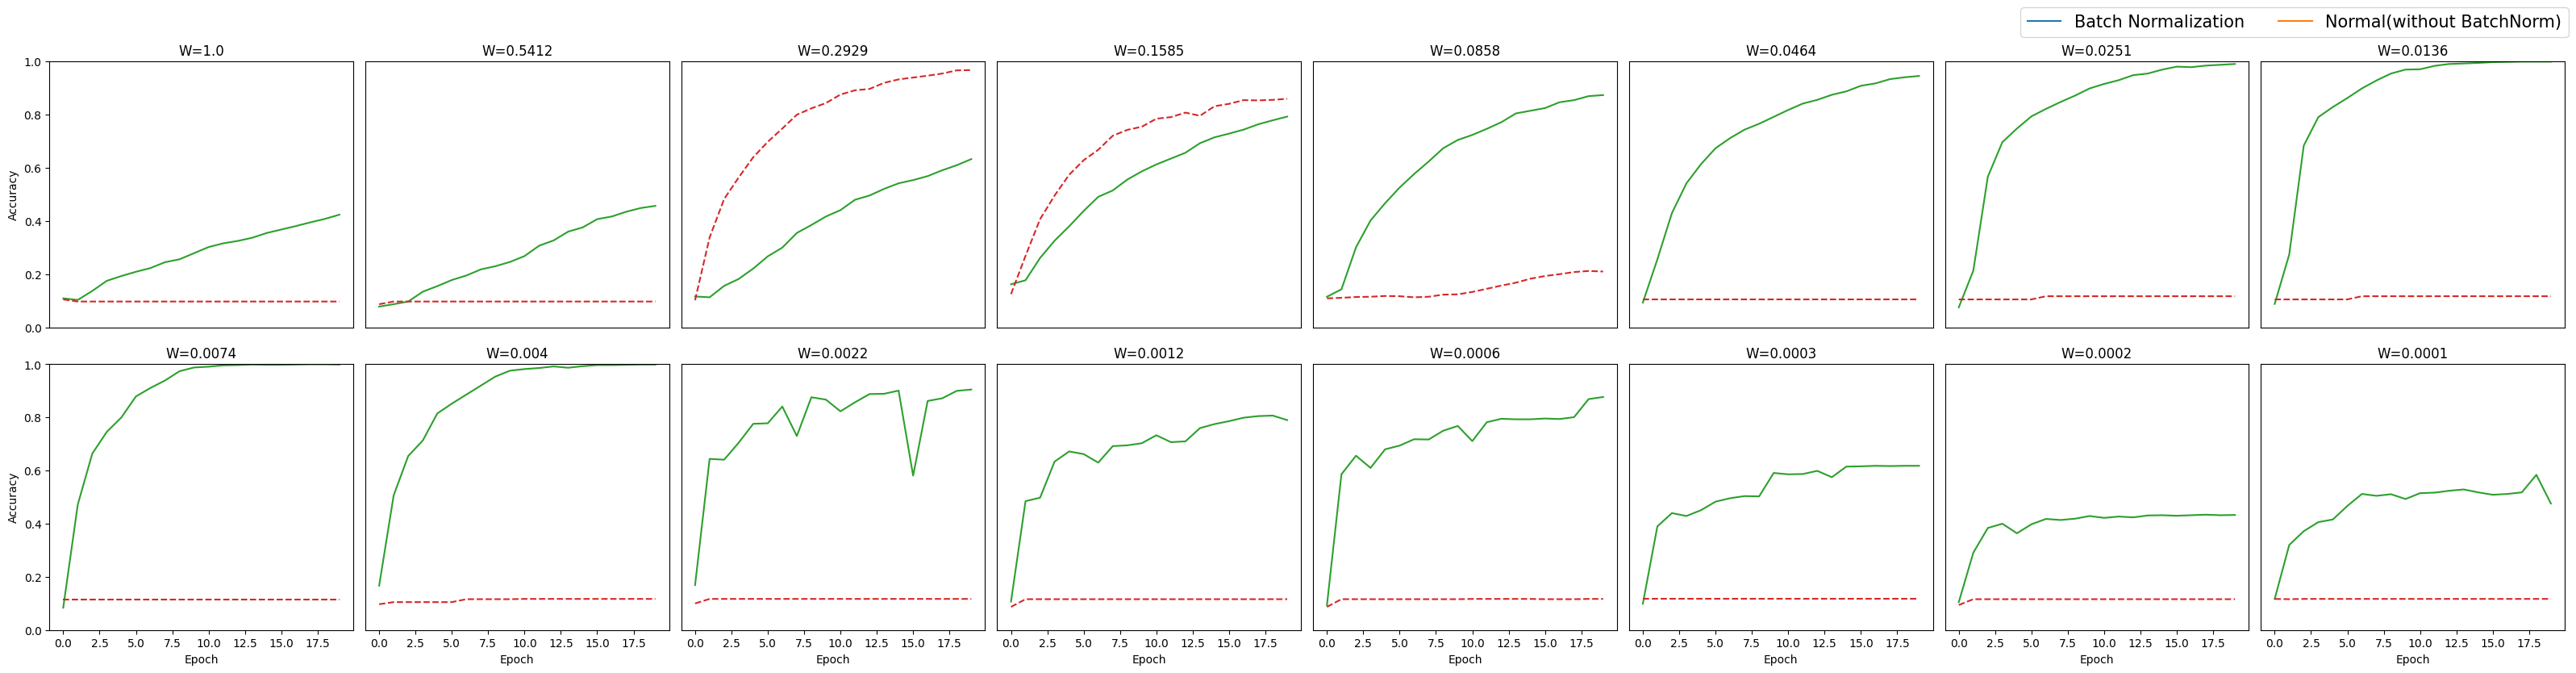
\includegraphics[width=\textwidth]{Figures/Use batch norm to compare with no use.png}
    \caption{Use batch norm to compare with no use}
    \label{Use batch norm to compare with no use}
\end{figure}

我们发现,几乎所有的情况下都是使用Batch Norm时学习进行得更快。
同时也可以发现,实际上,在不使用Batch Norm的情况下,如果不赋予一
个尺度好的初始值,学习将完全无法进行。

通过使用Batch Norm,可以推动学习的进行。并且,对权重初
始值变得健壮(“对初始值健壮”表示不那么依赖初始值)。
\section{正则化}
机器学习的问题中,过拟合是一个很常见的问题。过拟合指的是只能拟
合训练数据,但不能很好地拟合不包含在训练数据中的其他数据的状态。机
器学习的目标是提高泛化能力,即便是没有包含在训练数据里的未观测数据,
也希望模型可以进行正确的识别。我们可以制作复杂的、表现力强的模型,但是相应地,抑制过拟合的技巧也很重要。
\subsection{过拟合}
发生过拟合的原因,主要有以下两个:
\begin{enumerate}
    \item 模型拥有大量参数、表现力强。
    \item 训练数据少。
\end{enumerate}
\figures{Comparison of recognition accuracy between training data and test data}
\autoref{Comparison of recognition accuracy between training data and test data} 中,使用的数据量仅为300,神经网络的层数为7,这是故意满足过拟合条件的情况。
\subsection{权值衰减}
权值衰减是一直以来经常被使用的一种抑制过拟合的方法。该方法通过
在学习的过程中对大的权重进行惩罚,来抑制过拟合。很多过拟合原本就是
因为权重参数取值过大才发生的。
\begin{tcolorbox}
    $L_2$范数相当于各个元素的平方和。用数学式表示的话,假设有权重
    $W = (w_1, w_2, \cdots , w_n)$,则 $L_2$ 范数可用
    计算$\sqrt{w_1^2+w_2^2+\cdots+w_n^2}$出来。除了$L_2$范数,还有$L_1$范数、$L\infty$范数等。$L_1$范数是各个元
    素的绝对值之和,相当于$|w1| + |w2| + . . . + |wn|$。$L_{\infty}$范数也称为
    Max范数,相当于各个元素的绝对值中最大的那一个。$L_2$范数、$L_1$
    范数、$L_{\infty}$范数都可以用作正则化项,它们各有各的特点,不过这里
    我们要实现的是比较常用的$L_2$范数。
\end{tcolorbox}
\figures{Changes in recognition accuracy of training data and test data using weight decay}

\autoref{Changes in recognition accuracy of training data and test data using weight decay} 使用了权值衰退,这减少了过拟合现象,但是代价是降低了训练集的准确率,但是测试集的准确率没有任何的提升,也就是说这里的防止过拟合只是抑制训练集精度,模型似乎还是不是一个好的模型。
\subsection{Dropout}
作为抑制过拟合的方法,为损失函数加上权重的$L_2$范
数的权值衰减方法。该方法可以简单地实现,在某种程度上能够抑制过拟合。
但是,如果网络的模型变得很复杂,只用权值衰减就难以应对了。在这种情
况下,我们经常会使用\textbf{Dropout}方法。

Dropout是一种在学习的过程中随机删除神经元的方法。训练时,随机
选出隐藏层的神经元,然后将其删除。被删除的神经元不再进行信号的传递,
如 \autoref{Concept map of Dropout} 所示。训练时,每传递一次数据,就会随机选择要删除的神经元。
然后,测试时,虽然会传递所有的神经元信号,但是对于各个神经元的输出,
要乘上训练时的删除比例后再输出。

\figures{Concept map of Dropout}

\begin{figure}
    \centering
    \begin{subfigure}{.45\textwidth}
        \centering
        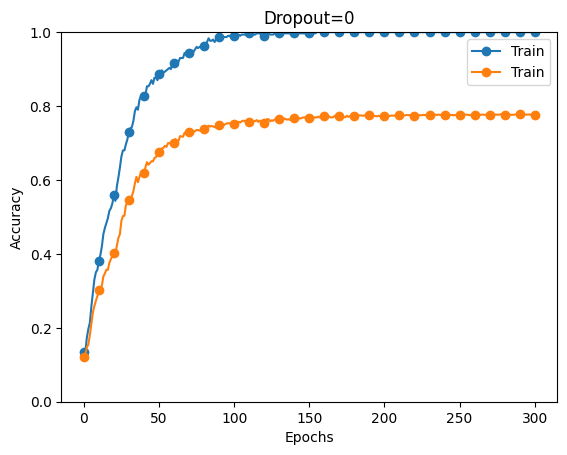
\includegraphics[width=\textwidth]{Figures/without dropout.png}
        \caption{$dropout = 0$}
        \label{dropout0}
    \end{subfigure}
    \hfill
    \begin{subfigure}{.45\textwidth}
        \centering
        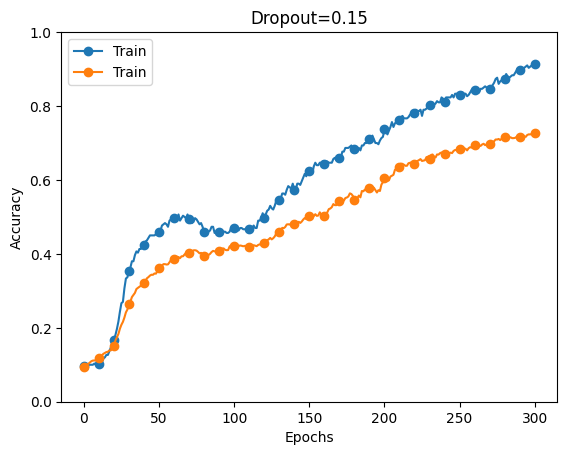
\includegraphics[width=\textwidth]{Figures/use dropout.png}
        \caption{$dropout = 0.15$}
        \label{dropout015}
    \end{subfigure}
    \caption{Comparison between dropout use or not}
    \label{Comparison between dropout use or not}
\end{figure}
\autoref{Comparison between dropout use or not} 中,通过使用Dropout,训练数据和测试数据的识别精度的差距
变小了。并且,训练数据也没有到达100\%的识别精度。像这样,通过使用
Dropout,即便是表现力强的网络,也可以抑制过拟合。
\begin{tcolorbox}
    集成学习与Dropout有密切的关系。这是因为可以将Dropout
    理解为,通过在学习过程中随机删除神经元,从而每一次都让不同
    的模型进行学习。并且,推理时,通过对神经元的输出乘以删除比
    例(比如,0.5等),可以取得模型的平均值。也就是说,可以理解成,
    Dropout将集成学习的效果(模拟地)通过一个网络实现了。
\end{tcolorbox}

\paragraph{一点补充} 为了对齐Dropout训练和预测的结果,通常有两种做法,假设dropout rate = 0.2。一种是训练时不做处理,预测时输出乘以(1 - dropout rate)。另一种是训练时留下的神经元除以(1 - dropout rate),预测时不做处理。(\href{https://www.cnblogs.com/jiangxinyang/p/14333903.html}{参考地址})
\section{超参数的验证}
神经网络中,除了权重和偏置等参数,超参数(hyper-parameter)也经
常出现。这里所说的超参数是指,比如各层的神经元数量、batch大小、参
数更新时的学习率或权值衰减等。如果这些超参数没有设置合适的值,模型
的性能就会很差。虽然超参数的取值非常重要,但是在决定超参数的过程中
一般会伴随很多的试错。
\subsection{验证数据}
这里要注意的是,
不能使用测试数据评估超参数的性能。这一点非常重要,但也容易被忽视。

为什么不能用测试数据评估超参数的性能呢?这是因为如果使用测试数
据调整超参数,超参数的值会对测试数据发生过拟合。换句话说,用测试数
据确认超参数的值的“好坏”,就会导致超参数的值被调整为只拟合测试数据。
这样的话,可能就会得到不能拟合其他数据、泛化能力低的模型。

因此,调整超参数时,必须使用超参数专用的确认数据。用于调整超参
数的数据,一般称为\textbf{验证数据}(validation data)。我们使用这个验证数据来评估超参数的好坏。
\begin{tcolorbox}
    训练数据用于参数(权重和偏置)的学习,验证数据用于超参数的性
    能评估。为了确认泛化能力,要在最后使用(比较理想的是只用一次)
    测试数据。
\end{tcolorbox}
\subsection{超参数的最优化}
进行超参数的最优化时,逐渐缩小超参数的“好值”的存在范围非常重要。
所谓逐渐缩小范围,是指一开始先大致设定一个范围,从这个范围中随机选
出一个超参数(采样),用这个采样到的值进行识别精度的评估;然后,多次
重复该操作,观察识别精度的结果,根据这个结果缩小超参数的“好值”的范围。
通过重复这一操作,就可以逐渐确定超参数的合适范围。
\begin{tcolorbox}
    有\href{https://www.jmlr.org/papers/volume13/bergstra12a/bergstra12a.pdf}{报告}显示,在进行神经网络的超参数的最优化时,与网格搜索
    等有规律的搜索相比,随机采样的搜索方式效果更好。这是因为在
    多个超参数中,各个超参数对最终的识别精度的影响程度不同。
\end{tcolorbox}

所谓“大致地指定”,是指
像 0.001($10^{-3}$)到 1000($10^3$)这样,以“10 的阶乘”的尺度指定范围(也表述为“用对数尺度(log scale)指定”)。

在超参数的最优化中,要注意的是深度学习需要很长时间(比如,几天
或几周)。因此,在超参数的搜索中,需要尽早放弃那些不符合逻辑的超参数。
于是,在超参数的最优化中,减少学习的epoch,缩短一次评估所需的时间
是一个不错的办法。
\begin{itemize}
    \item 步骤0:设定超参数的范围。
    \item 步骤1:从设定的超参数范围中随机采样。
    \item 步骤2:使用步骤1中采样到的超参数的值进行学习,通过验证数据评估识别精
          度(但是要将epoch设置得很小)。
    \item 步骤3:重复步骤1和步骤2(100次等),根据它们的识别精度的结果,缩小超参数的范围。
\end{itemize}

\begin{tcolorbox}
    这里介绍的超参数的最优化方法是实践性的方法。不过,这个方
    法与其说是科学方法,倒不如说有些实践者的经验的感觉。在超
    参数的最优化中,如果需要更精炼的方法,可以使用贝叶斯最优
    化(Bayesian optimization)。贝叶斯最优化运用以贝叶斯定理为中
    心的数学理论,能够更加严密、高效地进行最优化。详细内容请
    参 考 论 文“\href{https://arxiv.org/abs/1206.2944}{Practical Bayesian Optimization of Machine Learning Algorithms}”等。
\end{tcolorbox}
\subsection{超参数最优化的实现}
\figures{best 20 workouts}

\autoref{best 20 workouts} 展示最好的二十次训练,观察可以使学习顺利进行的超参
数的范围,从而缩小值的范围。然后,在这个缩小的范围中重复相同的操作。

\section{小结}
\begin{itemize}
    \item 参 数 的 更 新 方 法,除 了 SGD 之 外,还 有 Momentum、AdaGrad、
          Adam等方法。
    \item 权重初始值的赋值方法对进行正确的学习非常重要。
    \item 作为权重初始值,Xavier初始值、He初始值等比较有效。
    \item 通过使用Batch Normalization,可以加速学习,并且对初始值变得
          健壮。
    \item 抑制过拟合的正则化技术有权值衰减、Dropout等。
    \item 逐渐缩小“好值”存在的范围是搜索超参数的一个有效方法。
\end{itemize}
